\documentclass[hidelinks]{ctexart}

\usepackage[sensei=ない,gakka=計算化学,section=DFT,gakkabbr=CC]{styles/kurisu}
\usepackage{van-de-la-illinoise}

\DeclareSIUnit\bohr{Bohr}
\DeclareSIUnit\hatree{Hatree}

\hypersetup{
     colorlinks   = false,
     citecolor    = black
}

\newcommand{\numer}[1]{\SI{#1}{}}

\begin{document}

\bibliographystyle{unsrt}

\section{密度泛函理论\texorpdfstring{$\cdot$}{}笔记} % (fold)
\label{sec:密度汎関数理論}

\subsection{基本原理} % (fold)
\label{sub:基本原理}

\subsubsection{Kohn-Sham方程} % (fold)
\label{ssub:Kohn-Sham方程}

$\rho\pare{x,y,z}$(电子密度, \mgloss[-\baselineskip]{electron density})和单电子空间波函数(分子轨道)有关系
\[ \rho = \sum_{i=1}^n \abs{\psi_i}^2. \]
%对于闭壳层分子, 求和遍历$n$个轨道的一共$2n$个电子.
Kohn-Sham方程(\gloss{Kohn-Sham equation})为
\[ \brac{-\half \laplacian_i - \sum_{\text{核}A} \frac{Z_A}{r_{1A}} + \int \frac{\rho\pare{\+vr_2}}{r_{12}}\,\rd{\+vr_2} + v\+_XC_\pare{1}}\psi_i = \epsilon_i \psi_i\pare{1}. \]
\marginnote{\textit{疑问: 求解Kohn-Sham方程后得到的每个$\psi_i$应容纳一个电子还是两个电子?}}%
方括号内的算子为Kohn-Sham算子, 记作$\hat H\+_KS_$. 求解前需要选择基组$\curb{\phi_s}$并做展开
\[ \psi_i = \sum_{s=1}^m c_{si}\phi_s,\quad i = 1,2,\cdots, m, \]
则Kohn-Sham方程转化为
\[ \+vH\+vC = \+vS\+vC\+v\epsilon, \]
其中
\[ H_{lk} = \bra{\phi_l}\hat H\+_KS_\ket{\phi_k},\quad S_{lk} = \bra{\chi_l}\ket{\chi_k}. \]

% subsubsection Kohn-Sham方程 (end)

\subsubsection{求解步骤} % (fold)
\label{ssub:求解步骤}

求解能量的步骤如下\cite{Lewars2016}.
\begin{cenum}
    \item 指定几何构型(以及电荷, 重数等).
    \item 指定基函数$\curb{\phi}$和交换-关联泛函$E\+_XC_\brac{\rho}$.
    \item 猜测初始的$\rho$(例如叠加各原子的$\rho$).
    \item 通过$\rho$计算$v\+_XC_\pare{\+vr}$. 其中$v\+_XC_ = \delta E\+_XC_/\delta \rho$.
    \item 通过$\rho$和$v\+_XC_\pare{\+vr}$得到Kohn-Sham算子
    \[ \hat H^{\mathrm{KS}} = -\half \laplacian_i - \sum_{\text{核}A} \frac{Z\+_A_}{r\+_1A_} + \int \frac{\rho\pare{\+vr_2}}{r_{12}}\,\rd{\+vr_2} + v\+_XC_\pare{1}. \]
    \item 计算Kohn-Sham矩阵,\marginnote{\textit{疑问: 通常基函数的数量$m$大于电子数量$n$, 本征矢量$\+vC$的数目为$m$, 此时应当选取哪些列矢量$\+vC$组合成$\psi_i$? 是否如同在Hatree-Fock方法中那样选取$\epsilon$最低的本征矢量$\+vC$?}}
    \[ K_{rs} = \bra{\phi_r}\hat h^{\mathrm{KS}}\ket{\phi_s}. \]
    \item 将Kohn-Sham矩阵对角化, 得到系数矩阵$\+vC'$和能级$\+v\epsilon$, 并将$\+vC'$变回$\+vC$. 此时可得
    \[ \psi_i^{\mathrm{KS}} = \sum c \phi\+_basis_. \]
    \item 得到新的
    \[ \rho = \sum_{i=1}^{n}\abs{\psi_i^{\mathrm{KS}}\pare{1}}^2. \]
    \item 回到第四步. 若$\+v\epsilon$和$\psi_i$的变化不显著则可认为收敛. 否则须继续迭代.
    \item 迭代收敛后, 总能量
    \[ E_0 = -\sum_{\text{核}A} Z\+_A_\int \frac{\rho_0\pare{\+vr_1}}{\+vr\+_1A_}\,\rd{\+vr_1} - \half \sum_{i=1}^{2n}\bra{\psi_i^{\mathrm{KS}}\pare{1}}\laplacian_1\ket{\psi_i^{\mathrm{KS}}\pare{1}} + \half \iint \frac{\rho_0\pare{\+vr_1}\rho_0\pare{\+vr_2}}{r_{12}}\,\rd{\+vr_1}\,\rd{\+vr_2} + E\+_XC_\brac{\rho_0}. \]
    \item 取最小能量的构型, 可得构型优化.
\end{cenum}

% subsubsection 求解步骤 (end)

% subsection 基本原理 (end)

\subsection{交换-关联泛函} % (fold)
\label{sub:交换_关联泛函}

\subsubsection{LDA近似} % (fold)
\label{ssub:lda近似}

在局域密度近似(local-density approximations, \gloss{LDA})下(不考虑自旋极化),
\[ E\+_XC_\brac{\rho} = \int \rho\pare{\+vr}\epsilon\+_XC_\pare{\rho\pare{\+vr}}\,\rd{\+vr}. \]
其中$\epsilon\+_XC_$分为交换能和关联能两部分,
\[ \epsilon\+_XC_\pare{\rho} = \epsilon\+_x_\pare{\rho} + \epsilon\+_c_\pare{\rho}. \]
交换能取\cite{Thijssen2007}
\[ \epsilon\+_x_\pare{\rho} = -C\+_x_\rho^{1/3},\quad C\+_x_ = \frac{3}{4}\pare{\frac{3}{\pi}}^{1/3} = \SI{0.738559}{}. \]
关联能取Chachiyo泛函(\gloss{Chachiyo correlation functional})\cite{Chachiyo2016}
\[ \epsilon\+_c_\pare{\rho} = a \ln \pare{1 + \frac{b}{r_s} + \frac{b}{r_s^2}}, \]
其中\marginnote{\textit{疑问: SCF过程中每一步皆需要重新计算$\bra{\phi_i}v\+_XC_\ket{\phi_i}$, 而$\rho$的指数为$1/3$, 不能用$\phi_i$展开. 实际应用中除了数值积分外是否另有方法?}}
\[ a = \frac{\ln 2 - 1}{2\pi^2} = \SI{-0.0155453}{},\quad b = \SI{20.4562557}{},\quad r_s = \pare{\frac{4\pi \rho}{3}}^{-1/3}. \]
记
\[ b_1 = b \pare{\frac{4\pi}{3}}^{1/3} = \SI{32.9753}{},\quad b_2 = b\pare{\frac{4\pi}{3}}^{2/3} = \SI{53.1559}{}, \]
则
\begin{align*}
    E\+_XC_\brac{\rho} &= \int \pare{-C\+_x_ \rho^{1/3} + a\ln \pare{1+b_1 \rho^{1/3} + b_2\rho^{2/3}}}\rho\,\rd{\+vr}, \\
    v\+_XC_ &= \rec{3}\pare{-4C\+_x_ + \frac{a\pare{b_1 + 2b_2 \rho^{1/3}}}{1+b_1\rho^{1/3} + b_2\rho^{2/3}}}\rho^{1/3} + a\ln \pare{1+b_1 \rho^{1/3} + b_2 \rho^{2/3}}.
\end{align*}

% subsubsection lda近似 (end)

% subsection 交换_关联泛函 (end)

\subsection{基函数} % (fold)
\label{sub:基函数}

DFT中常用的基函数之一为6-31G\textsuperscript{*}. 最小基函数(minimal basis)之一为STO-3G.

\subsubsection{STO-3G基函数} % (fold)
\label{ssub:sto_3g基函数}

\gloss{STO-3G}基函数对1s轨道做如下展开:
\[ \psi = c_1\phi\+_1s_\pare{\alpha_1} + c_2\phi\+_1s_\pare{\alpha_2} + c_3\phi\+_1s_\pare{\alpha_3}, \]
其中$\phi$为1s的Gau\ss 型基函数,
\[ \phi\+_1s_\pare{\alpha} = \pare{\frac{2\alpha}{\pi}}^{3/4}e^{-\alpha r^2}. \]
记Slater基函数
\[ \phi^{\mathrm{Slater}}\+_1s_\pare{\zeta,\+vr} = \sqrt{\frac{\zeta^3}{\pi}}e^{-\zeta r}, \]
则如下拟合成立\cite{Hehre1969}
\[ \phi^{\mathrm{Slater}}\+_1s_\pare{\zeta = 1,\+vr} = \begin{cases}
    \SI{0.444635}{}\ \phi\+_1s_\pare{\SI{0.109818}{}}\\ + \SI{0.535328}{}\ \phi\+_1s_\pare{\SI{0.405771}{}} \\ + \SI{0.154329}{}\ \phi\+_1s_\pare{\SI{2.22766}{}}.\end{cases} \]
对于$\zeta\neq 1$的情形, 将上式中的各$\alpha$变为$\alpha \zeta^2$即可. 分子中的氢原子的1s轨道会略微收缩, $\zeta = 1.24$, 拟合为\cite{szabo1996modern}
\[ \phi^{\mathrm{Slater}}\+_1s_\pare{\zeta = 1.24,\+vr} = \begin{cases}
    \SI{0.444635}{}\ \phi\+_1s_\pare{\SI{0.168856}{}}\\ + \SI{0.535328}{}\ \phi\+_1s_\pare{\SI{0.623913}{}} \\ + \SI{0.154329}{}\ \phi\+_1s_\pare{\SI{3.42525}{}}.\end{cases} \]
对于氢分子系统, 设原子核分别位于$\+vR_1$, $\+vR_2$, $\abs{\+vR_1 - \+vR_2} = \SI{0.7414}{\angstrom} = \SI{1.400}{\bohr}$. 取6个基函数
\begin{flalign*}
    & && \phi_1 = \numer{0.187736}\ e^{\numer{-0.168856}\ \abs{\+vr - \+vR_1}^2}, && \phi_4 = \numer{0.187736}\ e^{\numer{-0.168856}\ \abs{\+vr - \+vR_2}^2}, && \\
    & && \phi_2 = \numer{0.500326}\ e^{\numer{-0.623913}\ \abs{\+vr - \+vR_1}^2}, && \phi_5 = \numer{0.500326}\ e^{\numer{-0.623913}\ \abs{\+vr - \+vR_2}^2}, && \\
    & && \phi_3 = \numer{1.79444}\ e^{\numer{-3.42525}\ \abs{\+vr - \+vR_1}^2}, && \phi_6 = \numer{1.79444}\ e^{\numer{-3.42525}\ \abs{\+vr - \+vR_2}^2}. &&
\end{flalign*}

% subsubsection sto_3g基函数 (end)

\subsubsection{交叠积分} % (fold)
\label{ssub:交叠积分}

对于1s类型的GTO, 可通过\cite{1980量子化学}
\[ \int e^{-ar\+_A_^2 - br\+_B_^2}\,\rd{\tau} = \exp\pare{-\frac{ab}{a+b}\abs{AB}^2}\pare{\frac{\pi}{a+b}}^{3/2} \]
计算其交叠积分.
\begin{align*}
    & S_{ij} = \bra{\phi_i}\ket{\phi_j} = \begin{pmatrix}
 1. & 0.740978 & 0.275306 & 0.847488 & 0.571067 & 0.200833 \\
 0.740978 & 1. & 0.613563 & 0.571067 & 0.542572 & 0.218075 \\
 0.275306 & 0.613563 & 1. & 0.200833 & 0.218075 & 0.0348485 \\
 0.847488 & 0.571067 & 0.200833 & 1. & 0.740978 & 0.275306 \\
 0.571067 & 0.542572 & 0.218075 & 0.740978 & 1. & 0.613563 \\
 0.200833 & 0.218075 & 0.0348485 & 0.275306 & 0.613563 & 1.
\end{pmatrix}. \\
    & {\+vS}^{1/2} = \begin{pmatrix}
 0.792108 & 0.364046 & 0.0721153 & 0.442248 & 0.192187 & 0.0481296 \\
 0.364046 & 0.822158 & 0.319765 & 0.192187 & 0.218523 & 0.0677382 \\
 0.0721153 & 0.319765 & 0.941051 & 0.0481296 & 0.0677382 & -0.0081897 \\
 0.442248 & 0.192187 & 0.0481296 & 0.792108 & 0.364046 & 0.0721153 \\
 0.192187 & 0.218523 & 0.0677382 & 0.364046 & 0.822158 & 0.319765 \\
 0.0481296 & 0.0677382 & -0.0081897 & 0.0721153 & 0.319765 & 0.941051
    \end{pmatrix}.
\end{align*}


% subsubsection 交叠积分 (end)

\subsubsection{动能积分} % (fold)
\label{ssub:动能积分}

对于1s类型的GTO, 可通过\cite{1980量子化学}
\[ T_{ij} = \bra{\phi_i}{-\half\laplacian}\ket{\phi_j} = \frac{\alpha_i \alpha_j}{\alpha_i + \alpha_j}\brac{3 - \frac{2\alpha_i \alpha_j}{\alpha_i + \alpha_j}\abs{AB}^2}S_{ij} \]
计算其动能积分.
\[ T_{ij} = \bra{\phi_i}{-\half\laplacian}\ket{\phi_j} = \begin{pmatrix}
0.253284 & 0.295407 & 0.132909 & 0.190975 & 0.188135 & 0.0765687 \\
 0.295407 & 0.93587 & 0.971475 & 0.188135 & 0.300795 & 0.107166 \\
 0.132909 & 0.971475 & 5.13788 & 0.0765687 & 0.107166 & -0.22163 \\
 0.190975 & 0.188135 & 0.0765687 & 0.253284 & 0.295407 & 0.132909 \\
 0.188135 & 0.300795 & 0.107166 & 0.295407 & 0.93587 & 0.971475 \\
 0.0765687 & 0.107166 & -0.22163 & 0.132909 & 0.971475 & 5.13788
\end{pmatrix}. \]

% subsubsection 动能积分 (end)

\subsubsection{核-电子积分} % (fold)
\label{ssub:核_电子积分}

对于1s类型的GTO, 可通过\cite{1980量子化学}
\[ \int e^{-ar\+_A_^2 - br\+_B_^2}\rec{r\+_C_}\,\rd{\tau} = \exp\pare{-\frac{ab}{a+b}\abs{AB}^2}\frac{2\pi}{a+b}F_0\brac{\pare{a+b}\abs{PC}^2} \]
计算其核-电子积分, 其中
\[ \+vR_P = \frac{a\+vR_A + b\+vR_B}{a+b}, \]
而$F_0$为不完全$\Gamma$函数,
\[ F_m\pare{w} = \int_0^1 \exp\pare{-wt^2}t^{2m}\,\rd{t}. \]
\begin{align*}
    &V^{\mathrm{N}}_{ij} = \bra{\phi_i}{-\rec{\abs{\+vr-\+vR_1}} - \rec{\abs{\+vr-\+vR_2}}}\ket{\phi_j}\\ &= \begin{pmatrix}
 -1.19152 & -1.23247 & -0.785546 & -1.05307 & -0.99315 & -0.577876 \\
 -1.23247 & -1.95548 & -1.83138 & -0.99315 & -1.13351 & -0.649742 \\
 -0.785546 & -1.83138 & -3.66764 & -0.577876 & -0.649742 & -0.0986144 \\
 -1.05307 & -0.99315 & -0.577876 & -1.19152 & -1.23247 & -0.785546 \\
 -0.99315 & -1.13351 & -0.649742 & -1.23247 & -1.95548 & -1.83138 \\
 -0.577876 & -0.649742 & -0.0986144 & -0.785546 & -1.83138 & -3.66764
\end{pmatrix}.
\end{align*}

% subsubsection 核_电子积分 (end)

\subsubsection{电子-电子积分} % (fold)
\label{ssub:电子_电子积分}

记
\begin{align*}
    \pare{ij\vert kl} &= \iint \phi^*_i\pare{\+vr_1}\phi^*_k\pare{\+vr_2} \rec{r_{12}}\phi_j\pare{\+vr_1}\phi_l\pare{\+vr_2}\,\rd{\tau_1}\,\rd{\tau_2}\\ &= \iint \phi_i\pare{\+vr_1}\phi_j\pare{\+vr_1} \rec{r_{12}}\phi_k\pare{\+vr_2}\phi_l\pare{\+vr_2}\,\rd{\tau_1}\,\rd{\tau_2},
\end{align*}
其中第二个等号对于实数的$\phi$成立. 对于实数的$\phi$还成立
\[ \pare{ij\vert kl} = \pare{ji\vert kl} = \pare{ij\vert lk} = \pare{ji\vert lk} = \pare{kl\vert ij} = \pare{kl\vert ji} = \pare{lk\vert ij} = \pare{lk\vert ji}. \]
考虑到这一对称性后, 对于规模为$6$的基, 仍需计算$231$个积分. 对于氢原子, 由于两个原子的基函数相同, 实际上独立的积分更少.
\par
对于1s类型的GTO, 可通过\cite{1980量子化学}
\begin{align*}
    & \iint e^{-ar\+_A1_^2 - br\+_B1_^2}\rec{r_{12}}e^{-cr\+_C2_^2 - dr\+_D2_^2}\,\rd{\tau_1}\,\rd{\tau_2}, \\
    & = \frac{2\pi^{5/2}}{\pare{a+b}\pare{c+d}\sqrt{a+b+c+d}}\exp{-\frac{ab}{a+b}\abs{AB}^2 - \frac{cd}{c+d}\abs{CD}^2}F_0\brac{\frac{\abs{PQ}^2 \pare{a+b}\pare{c+d}}{a+b+c+d}}.
\end{align*}
计算多中心积分, 其中
\[ \+vR_P = \frac{a\+vR_A + b\+vR_B}{a+b},\quad \+vR_Q = \frac{c\+vR_C + d\+vR_D}{c+d}. \]
将积分结果列出如下.
\begin{longtable}{cccccccc}
    (1,1,1,1) & 
0.463675
 & 
(1,1,1,2) & 
0.406888
 & 
(1,1,1,3) & 
0.172601
 & 
(1,1,1,4) & 
0.382385
\\
(1,1,1,5) & 
0.285958
 & 
(1,1,1,6) & 
0.1062
 & 
(1,2,1,2) & 
0.390054
 & 
(1,2,1,3) & 
0.18551
\\
(1,2,1,4) & 
0.331946
 & 
(1,2,1,5) & 
0.258626
 & 
(1,2,1,6) & 
0.0972203
 & 
(1,3,1,3) & 
0.114648
\\
(1,3,1,4) & 
0.139224
 & 
(1,3,1,5) & 
0.11284
 & 
(1,3,1,6) & 
0.0409667
 & 
(1,4,1,4) & 
0.333028
\\
(1,4,1,5) & 
0.262412
 & 
(1,4,1,6) & 
0.102451
 & 
(1,5,1,5) & 
0.231679
 & 
(1,5,1,6) & 
0.103089
\\
(1,6,1,6) & 
0.0610106
 & 
(1,1,2,2) & 
0.581724
 & 
(1,1,2,3) & 
0.386538
 & 
(1,1,2,4) & 
0.311399
\\
(1,1,2,5) & 
0.302445
 & 
(1,1,2,6) & 
0.119738
 & 
(1,2,2,2) & 
0.582147
 & 
(1,2,2,3) & 
0.417702
\\
(1,2,2,4) & 
0.297117
 & 
(1,2,2,5) & 
0.292533
 & 
(1,2,2,6) & 
0.112885
 & 
(1,3,2,2) & 
0.298974
\\
(1,3,2,3) & 
0.263008
 & 
(1,3,2,4) & 
0.140266
 & 
(1,3,2,5) & 
0.140684
 & 
(1,3,2,6) & 
0.0496391
\\
(1,4,2,2) & 
0.472413
 & 
(1,4,2,3) & 
0.311645
 & 
(1,4,2,4) & 
0.262412
 & 
(1,4,2,5) & 
0.26749
\\
(1,4,2,6) & 
0.113656
 & 
(1,5,2,2) & 
0.374232
 & 
(1,5,2,3) & 
0.252964
 & 
(1,5,2,4) & 
0.21334
\\
(1,5,2,5) & 
0.237224
 & 
(1,5,2,6) & 
0.114246
 & 
(1,6,2,2) & 
0.140081
 & 
(1,6,2,3) & 
0.0915041
\\
(1,6,2,4) & 
0.0843891
 & 
(1,6,2,5) & 
0.105145
 & 
(1,6,2,6) & 
0.0672314
 & 
(1,1,3,3) & 
0.640146
\\
(1,1,3,4) & 
0.125854
 & 
(1,1,3,5) & 
0.136724
 & 
(1,1,3,6) & 
0.0211889
 & 
(1,2,3,3) & 
0.704783
\\
(1,2,3,4) & 
0.135201
 & 
(1,2,3,5) & 
0.146949
 & 
(1,2,3,6) & 
0.0219849
 & 
(1,3,3,3) & 
0.476959
\\
(1,3,3,4) & 
0.0834183
 & 
(1,3,3,5) & 
0.0907901
 & 
(1,3,3,6) & 
0.0119441
 & 
(1,4,3,3) & 
0.515297
\\
(1,4,3,4) & 
0.102451
 & 
(1,4,3,5) & 
0.113656
 & 
(1,4,3,6) & 
0.0189059
 & 
(1,5,3,3) & 
0.420326
\\
(1,5,3,4) & 
0.0843891
 & 
(1,5,3,5) & 
0.097317
 & 
(1,5,3,6) & 
0.0182291
 & 
(1,6,3,3) & 
0.149957
\\
(1,6,3,4) & 
0.0312831
 & 
(1,6,3,5) & 
0.0380185
 & 
(1,6,3,6) & 
0.00917591
 & 
(1,1,4,4) & 
0.417225
\\
(1,1,4,5) & 
0.351811
 & 
(1,1,4,6) & 
0.143295
 & 
(1,2,4,4) & 
0.351811
 & 
(1,2,4,5) & 
0.308812
\\
(1,2,4,6) & 
0.1296
 & 
(1,3,4,4) & 
0.143295
 & 
(1,3,4,5) & 
0.1296
 & 
(1,3,4,6) & 
0.0537076
\\
(1,4,4,4) & 
0.382385
 & 
(1,4,4,5) & 
0.331946
 & 
(1,4,4,6) & 
0.139224
 & 
(1,5,4,4) & 
0.311399
\\
(1,5,4,5) & 
0.297117
 & 
(1,5,4,6) & 
0.140266
 & 
(1,6,4,4) & 
0.125854
 & 
(1,6,4,5) & 
0.135201
\\
(1,6,4,6) & 
0.0834183
 & 
(1,1,5,5) & 
0.494722
 & 
(1,1,5,6) & 
0.320375
 & 
(1,2,5,5) & 
0.440331
\\
(1,2,5,6) & 
0.290012
 & 
(1,3,5,5) & 
0.185494
 & 
(1,3,5,6) & 
0.119896
 & 
(1,4,5,5) & 
0.472413
\\
(1,4,5,6) & 
0.311645
 & 
(1,5,5,5) & 
0.442292
 & 
(1,5,5,6) & 
0.315704
 & 
(1,6,5,5) & 
0.217808
\\
(1,6,5,6) & 
0.191336
 & 
(1,1,6,6) & 
0.527613
 & 
(1,2,6,6) & 
0.47892
 & 
(1,3,6,6) & 
0.196182
\\
(1,4,6,6) & 
0.515297
 & 
(1,5,6,6) & 
0.531945
 & 
(1,6,6,6) & 
0.346758
 & 
(2,2,2,2) & 
0.891286
\\
(2,2,2,3) & 
0.676176
 & 
(2,2,2,4) & 
0.442292
 & 
(2,2,2,5) & 
0.438516
 & 
(2,2,2,6) & 
0.165378
\\
(2,3,2,3) & 
0.604424
 & 
(2,3,2,4) & 
0.315704
 & 
(2,3,2,5) & 
0.316913
 & 
(2,3,2,6) & 
0.111042
\\
(2,4,2,4) & 
0.231679
 & 
(2,4,2,5) & 
0.237224
 & 
(2,4,2,6) & 
0.097317
 & 
(2,5,2,5) & 
0.262381
\\
(2,5,2,6) & 
0.121291
 & 
(2,6,2,6) & 
0.0763545
 & 
(2,2,3,3) & 
1.1593
 & 
(2,2,3,4) & 
0.217808
\\
(2,2,3,5) & 
0.23682
 & 
(2,2,3,6) & 
0.0343946
 & 
(2,3,3,3) & 
1.10446
 & 
(2,3,3,4) & 
0.191336
\\
(2,3,3,5) & 
0.208267
 & 
(2,3,3,6) & 
0.0270547
 & 
(2,4,3,3) & 
0.531945
 & 
(2,4,3,4) & 
0.103089
\\
(2,4,3,5) & 
0.114246
 & 
(2,4,3,6) & 
0.0182291
 & 
(2,5,3,3) & 
0.535505
 & 
(2,5,3,4) & 
0.105145
\\
(2,5,3,5) & 
0.121291
 & 
(2,5,3,6) & 
0.0219198
 & 
(2,6,3,3) & 
0.182752
 & 
(2,6,3,4) & 
0.0380185
\\
(2,6,3,5) & 
0.0465816
 & 
(2,6,3,6) & 
0.0113836
 & 
(2,2,4,4) & 
0.494722
 & 
(2,2,4,5) & 
0.440331
\\
(2,2,4,6) & 
0.185494
 & 
(2,3,4,4) & 
0.320375
 & 
(2,3,4,5) & 
0.290012
 & 
(2,3,4,6) & 
0.119896
\\
(2,4,4,4) & 
0.285958
 & 
(2,4,4,5) & 
0.258626
 & 
(2,4,4,6) & 
0.11284
 & 
(2,5,4,4) & 
0.302445
\\
(2,5,4,5) & 
0.292533
 & 
(2,5,4,6) & 
0.140684
 & 
(2,6,4,4) & 
0.136724
 & 
(2,6,4,5) & 
0.146949
\\
(2,6,4,6) & 
0.0907901
 & 
(2,2,5,5) & 
0.630111
 & 
(2,2,5,6) & 
0.414966
 & 
(2,3,5,5) & 
0.414966
\\
(2,3,5,6) & 
0.267597
 & 
(2,4,5,5) & 
0.374232
 & 
(2,4,5,6) & 
0.252964
 & 
(2,5,5,5) & 
0.438516
\\
(2,5,5,6) & 
0.316913
 & 
(2,6,5,5) & 
0.23682
 & 
(2,6,5,6) & 
0.208267
 & 
(2,2,6,6) & 
0.684331
\\
(2,3,6,6) & 
0.437564
 & 
(2,4,6,6) & 
0.420326
 & 
(2,5,6,6) & 
0.535505
 & 
(2,6,6,6) & 
0.377592
\\
(3,3,3,3) & 
2.08834
 & 
(3,3,3,4) & 
0.346758
 & 
(3,3,3,5) & 
0.377592
 & 
(3,3,3,6) & 
0.0464516
\\
(3,4,3,4) & 
0.0610106
 & 
(3,4,3,5) & 
0.0672314
 & 
(3,4,3,6) & 
0.00917591
 & 
(3,5,3,5) & 
0.0763545
\\
(3,5,3,6) & 
0.0113836
 & 
(3,6,3,6) & 
0.00253612
 & 
(3,3,4,4) & 
0.527613
 & 
(3,3,4,5) & 
0.47892
\\
(3,3,4,6) & 
0.196182
 & 
(3,4,4,4) & 
0.1062
 & 
(3,4,4,5) & 
0.0972203
 & 
(3,4,4,6) & 
0.0409667
\\
(3,5,4,4) & 
0.119738
 & 
(3,5,4,5) & 
0.112885
 & 
(3,5,4,6) & 
0.0496391
 & 
(3,6,4,4) & 
0.0211889
\\
(3,6,4,5) & 
0.0219849
 & 
(3,6,4,6) & 
0.0119441
 & 
(3,3,5,5) & 
0.684331
 & 
(3,3,5,6) & 
0.437564
\\
(3,4,5,5) & 
0.140081
 & 
(3,4,5,6) & 
0.0915041
 & 
(3,5,5,5) & 
0.165378
 & 
(3,5,5,6) & 
0.111042
\\
(3,6,5,5) & 
0.0343946
 & 
(3,6,5,6) & 
0.0270547
 & 
(3,3,6,6) & 
0.714109
 & 
(3,4,6,6) & 
0.149957
\\
(3,5,6,6) & 
0.182752
 & 
(3,6,6,6) & 
0.0464516
 & 
(4,4,4,4) & 
0.463675
 & 
(4,4,4,5) & 
0.406888
\\
(4,4,4,6) & 
0.172601
 & 
(4,5,4,5) & 
0.390054
 & 
(4,5,4,6) & 
0.18551
 & 
(4,6,4,6) & 
0.114648
\\
(4,4,5,5) & 
0.581724
 & 
(4,4,5,6) & 
0.386538
 & 
(4,5,5,5) & 
0.582147
 & 
(4,5,5,6) & 
0.417702
\\
(4,6,5,5) & 
0.298974
 & 
(4,6,5,6) & 
0.263008
 & 
(4,4,6,6) & 
0.640146
 & 
(4,5,6,6) & 
0.704783
\\
(4,6,6,6) & 
0.476959
 & 
(5,5,5,5) & 
0.891286
 & 
(5,5,5,6) & 
0.676176
 & 
(5,6,5,6) & 
0.604424
\\
(5,5,6,6) & 
1.1593
 & 
(5,6,6,6) & 
1.10446
 & 
(6,6,6,6) & 
2.08834
 & 
\end{longtable}

% subsubsection 电子_电子积分 (end)

% subsection 基函数 (end)

\subsection{迭代求解} % (fold)
\label{sub:迭代求解}

\subsubsection{本征系统的求解} % (fold)
\label{ssub:本征系统的求解}

为了求解$\+vH\+vC = \+vS\+vC\+v\epsilon$, 令$\+vC' = \+vS^{1/2}\+vC$, $\+vH' = \pare{\+vS^{-1/2}}^T\+vH\+vS^{-1/2}$, 问题即转化为
\[ \+vH'\+vC' = \+vC'\+v\epsilon. \]
选择正交归一的$\+vC'$, 算得$\+vC$后组合成相应的$\psi$也是归一化的.

% subsubsection 本征系统的求解 (end)

\subsubsection{电荷密度与电子-电子积分} % (fold)
\label{ssub:电荷密度与电子_电子积分}

\begin{figure}[ht]
    \centering
    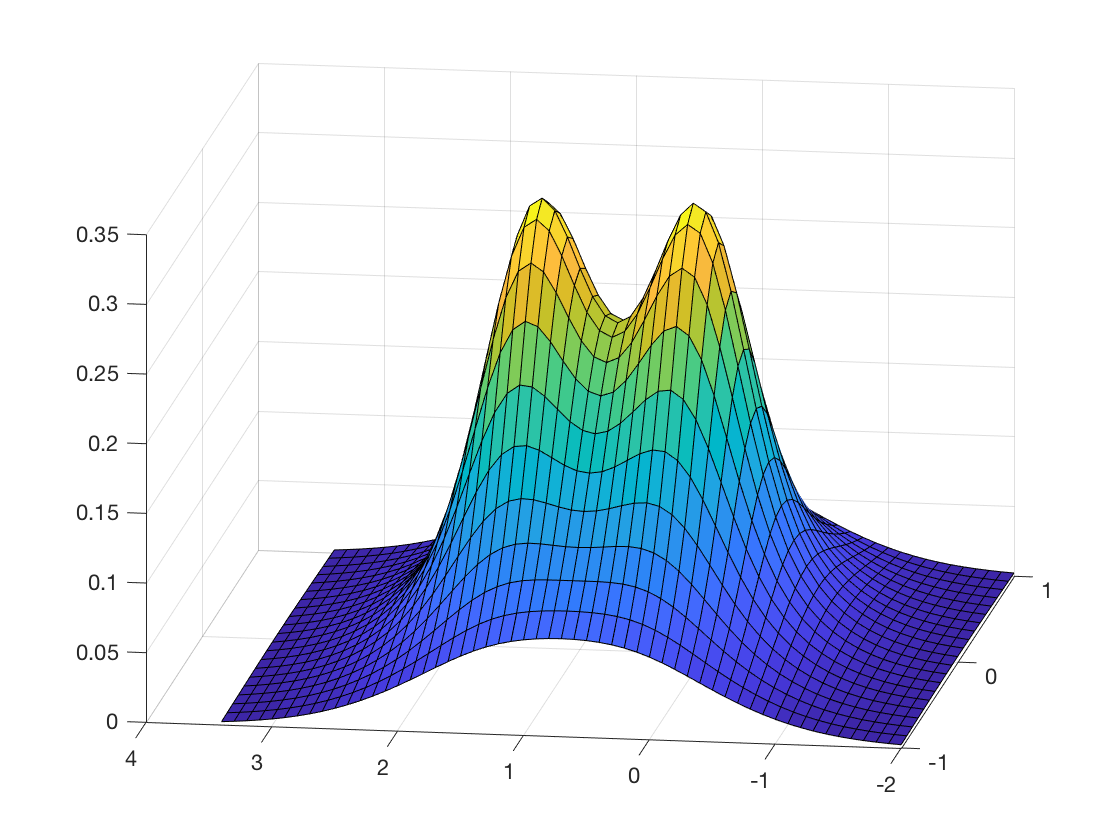
\includegraphics[width=8cm]{src/H2rho.png}
    \caption{STO-3G基得到的氢分子电荷密度}
\end{figure}

密度矩阵为
\[ P_{ij} = \sum_{k} n_k C_{ik} C^*_{jk} = \+vC \begin{pmatrix}
    n_1 & & & \\
    & n_2 & & \\
    & & \ddots & \\
    & & & n_k
\end{pmatrix} \+vC^\dagger. \]
可得电荷密度
\[ \rho\pare{\+vr} = \sum_{ij} P_{ij}\phi_i\pare{\+vr}\phi_j\pare{\+vr}, \]
以及相应的二电子积分
\[ \bra{\phi_i}\int \frac{\rho\pare{\+vr_2}}{r_{12}}\,\rd{\+vr_2}\,\ket{\phi_j} = \sum_{kl} P_{kl}\pare{ij\vert kl}. \]

% subsubsection 电荷密度与电子_电子积分 (end)

\subsubsection{总能量的获得} % (fold)
\label{ssub:总能量的获得}

总能量为(加上原子核的排斥能)\cite{Thijssen2007}
\[ E = \sum_{k=1}^n \epsilon_k - \half \iint \frac{\rho\pare{\+vr}\rho\pare{\+vr'}}{\abs{\+vr-\+vr'}}\,\rd{\+vr_1}\,\rd{\+vr_2} + E\+_XC_\brac{\rho} - \int v\+_XC_\brac{\rho} \rho\pare{\+vr}\,\rd{\+vr} + \sum_{\text{核}A,B} \frac{Z\+_A_Z\+_B_}{r\+_AB_}. \]
其中涉及电子-电子积分的项可写为
\[ -\half \iint \frac{\rho\pare{\+vr}\rho\pare{\+vr'}}{\abs{\+vr-\+vr'}}\,\rd{\+vr_1}\,\rd{\+vr_2} = -\half \sum_{ijkl}\pare{ij\vert kl}P_{ij}P_{kl}. \]
对于氢分子系统, STO-3G基给出$E = -\SI{1.122}{\hatree}$, 即解离能$\SI{0.122}{\hatree}$. 实际解离能$\SI{0.166}{\hatree}$.

% subsubsection 总能量的获得 (end)

% subsection 迭代求解 (end)

\subsection{参考文献} % (fold)
\label{sub:参考文献}

\renewcommand{\section}[2]{}%
\bibliography{DensityFunctionalTheory}
\href{https://github.com/Chen-Ze/ComputationalChemistry}{\color{blue!50!black}\textit{\,氢分子算例的源代码.}}

% subsection 参考文献 (end)

% section 密度汎関数理論 (end)

\end{document}
